\documentclass{chi2009}
\usepackage{times}
\usepackage{url}
\usepackage{graphics}
\usepackage{color}
\usepackage[pdftex]{hyperref}
\usepackage{algorithm}
\usepackage[noend]{algpseudocode}
\hypersetup{%
pdftitle={HybridPerfopticon: Query Visualization for Hybrid Distributed Databases},
pdfauthor={Brandon Haynes \& Shrainik Jain},
bookmarksnumbered,
pdfstartview={FitH},
colorlinks,
citecolor=black,
filecolor=black,
linkcolor=black,
urlcolor=black,
breaklinks=true,
}
\newcommand{\comment}[1]{}
\definecolor{Orange}{rgb}{1,0.5,0}
\definecolor{Green}{rgb}{0,1,0}
\definecolor{Blue}{rgb}{0,0,1}
\newcommand{\todo}[1]{\textsf{\textbf{\textcolor{Orange}{[[#1]]}}}}
\newcommand{\brandon}[1]{\textsf{\textbf{\textcolor{Blue}{[[#1]]}}}}
\newcommand{\shrainik}[1]{\textsf{\textbf{\textcolor{Green}{[[#1]]}}}}
\newcommand{\ea}{{\em et~al.} }
\newcommand{\ie}{{i.e.} }
\newcommand{\eg}{{e.g.}}

\pagenumbering{arabic}

\begin{document}
\special{papersize=8.5in,11in}
\setlength{\paperheight}{11in}
\setlength{\paperwidth}{8.5in}
\setlength{\pdfpageheight}{\paperheight}
\setlength{\pdfpagewidth}{\paperwidth}

\toappear{}

\title{HybridPerfopticon: Query Visualization for Hybrid Distributed Databases}
\numberofauthors{1} 
\author{\alignauthor Brandon Haynes \hspace{3em} Shrainik Jain \\
\affaddr{University of Washington} \\
\email{\{bhaynes, shrainik\}@cs.washington.edu}
} 

\maketitle

\begin{abstract}
Hybrid databases have recently gained a lot of attention because of the promise they show in several prominent use cases in scientific data management. A hybrid distributed database system usually consists of multiple underlying databases with differing data models. In order to better understand such systems we present a query profiling and visualization tool for queries authored over these hybrid systems. Our approach is to extend an existing visualization tool for distributed databases  by adding support for multiple underlying database systems.
\end{abstract}

\keywords{Hybrid Databases, Query Visualization} 

\category{H.5.2}{Graphical user interfaces (GUI)}{Miscellaneous}

\section{Introduction}
Stonebraker \ea \cite{stonebraker2007end} recently observed that the "one size fits all" era is over, and that the demands of big data management warrant a more federated approach to database design. Accordingly, "hybrid databases" -- generally dissimilar database management systems (DBMSs) combined in various ways -- are quickly emerging as an active area in database research. 

There exist many nascent examples of these hybrid DBMSs.  For example, Lim \ea in Cyclops \cite{cyclops} offers a top-down approach that combines compatible systems into a monolithic whole. Polybase \cite{polybase}, on the other hand, elected a bottom-up approach where disparate systems were more loosely coupled. 

To aid in understanding, development and debugging of these new systems, it would be advantageous to have visualization tools targeted at this class of DBMS. Unfortunately, most current profiling systems target queries in only a single database system. For example, SQL Server, Postgres, and MySQL all have a basic `explain' functionality, which displays a query plan in a human-readable (but often arcane) format.  Most `explain'-type tools lack deeper analysis features such as the ability to view performance over the duration of the query.  Further compounding this problem is the limited availability of tools available in a distributed database context, where operator-worker assignments, data skew, and similar problems are much more important.

Some tools, however, have been recently introduced that attempt to fill this need in a distributed database environment. Gprof \cite{gprof} is a basic visualization tool for system development.  However, it tends to be oriented toward developers.  Dapper \cite{dapper} is Google's production tracing tool designed to aid in distributed system development, but it lacks support for distributed query visualization.  Finally, Ambrose \cite{ambrose} is a framework designed to visualize map-reduce jobs.  While it offers many of the features that one would like to see in a robust distributed database visualization tool it currently targets only the map-reduce space and is not (in its current form) generalizable to a more broad set of DBMSs.

Compounding this is the fact that each of these tools lacks a complete visualization story where the tool is broadly useful across both users and system developers.  This has resulted in a scarcity of debugging and visualization in the distributed database space (and as a consequence the hybrid database space). 

To date, the Perfopticon \cite{perfopticon} system is the only system that is broadly-usable by various audiences and also addresses the profiling requirements of distributed database systems.  Perfopticon currently profiles queries on the Myria DBMS \cite{myria}, and can be used to profile similar relational systems.  However, while Perfopticon is able to be extended to other systems, it is not designed to \textit{simultaneously} display the results of queries that cross DBMS boundaries.

Accordingly, in this paper we present an extension to Perfopticon (aptly named "HybridPerfopticon") designed to expose support for the emerging hybrid use-case, where users require robust profiling of plans that co-occur across multiple database systems.  This class of queries present a number of unique challenges, such as how to display non-relational features (\eg, array chunks) in a framework that has heretofore targeted only tuple-based relational systems.  Additionally, a number of corollary challenges arise including coordinating the display of multiple sub-plans, visualizing data transfer between systems, and gathering profiling data from multiple sources.

For the purpose of demonstration, we created a hybrid distributed database system using SciDB \cite{scidb} and Myria \cite{Myria} as its component systems. SciDB's array-oriented data model is quite dissimilar from Myria's, making it critical to identify equivalent semantics for communication between these two systems. HybridPerfopticon highlights this communication by helping to visualize the overall hybrid query plan, tuple (and array element) flow between operators, skew in distribution of workloads among the constituent systems, and internal query time statistics.  It exposes these additional functions while maintaining complete compatibility with the existing underlying design.

In the next section, we present the architecture of the HybridPerfopticon system, which details the steps necessary to orchestrate hybrid plan execution and create Perfopticon-compatible hybrid plans for visualization purposes. This is followed by some results from the use case analysis. We conclude by looking at some future extensions to HybridPerfopticon.

\section{HybridPerfopticon Architecture}

Our approach to extending Perfopticon to support hybrid queries involved three major additions:

\begin{itemize}
\item Generating HybridPerfopticon-compatible SciDB plans
\item Creating HybridPerfopticon by extending Perfopticon to recognize components from varying underlying DBMSs
\item Creating hybrid plans and exposing them to HybridPerfopticon
\end{itemize}

In this section we describe each of these changes in detail and highlight the trade-offs in our design decisions.

\subsection{Generating SciDB Plans \& Metrics}

Perfopticon was initially designed to profile plans in the Myria DBMS \cite{perfopticon}.  In the Myria DBMS, each operator is instrumented to store profiling data.  When Perfopticon needs this profiling data, a HTTP request is generated, a query is performed over these data, and the aggregated results are returned.  
\begin{figure*}
\centering
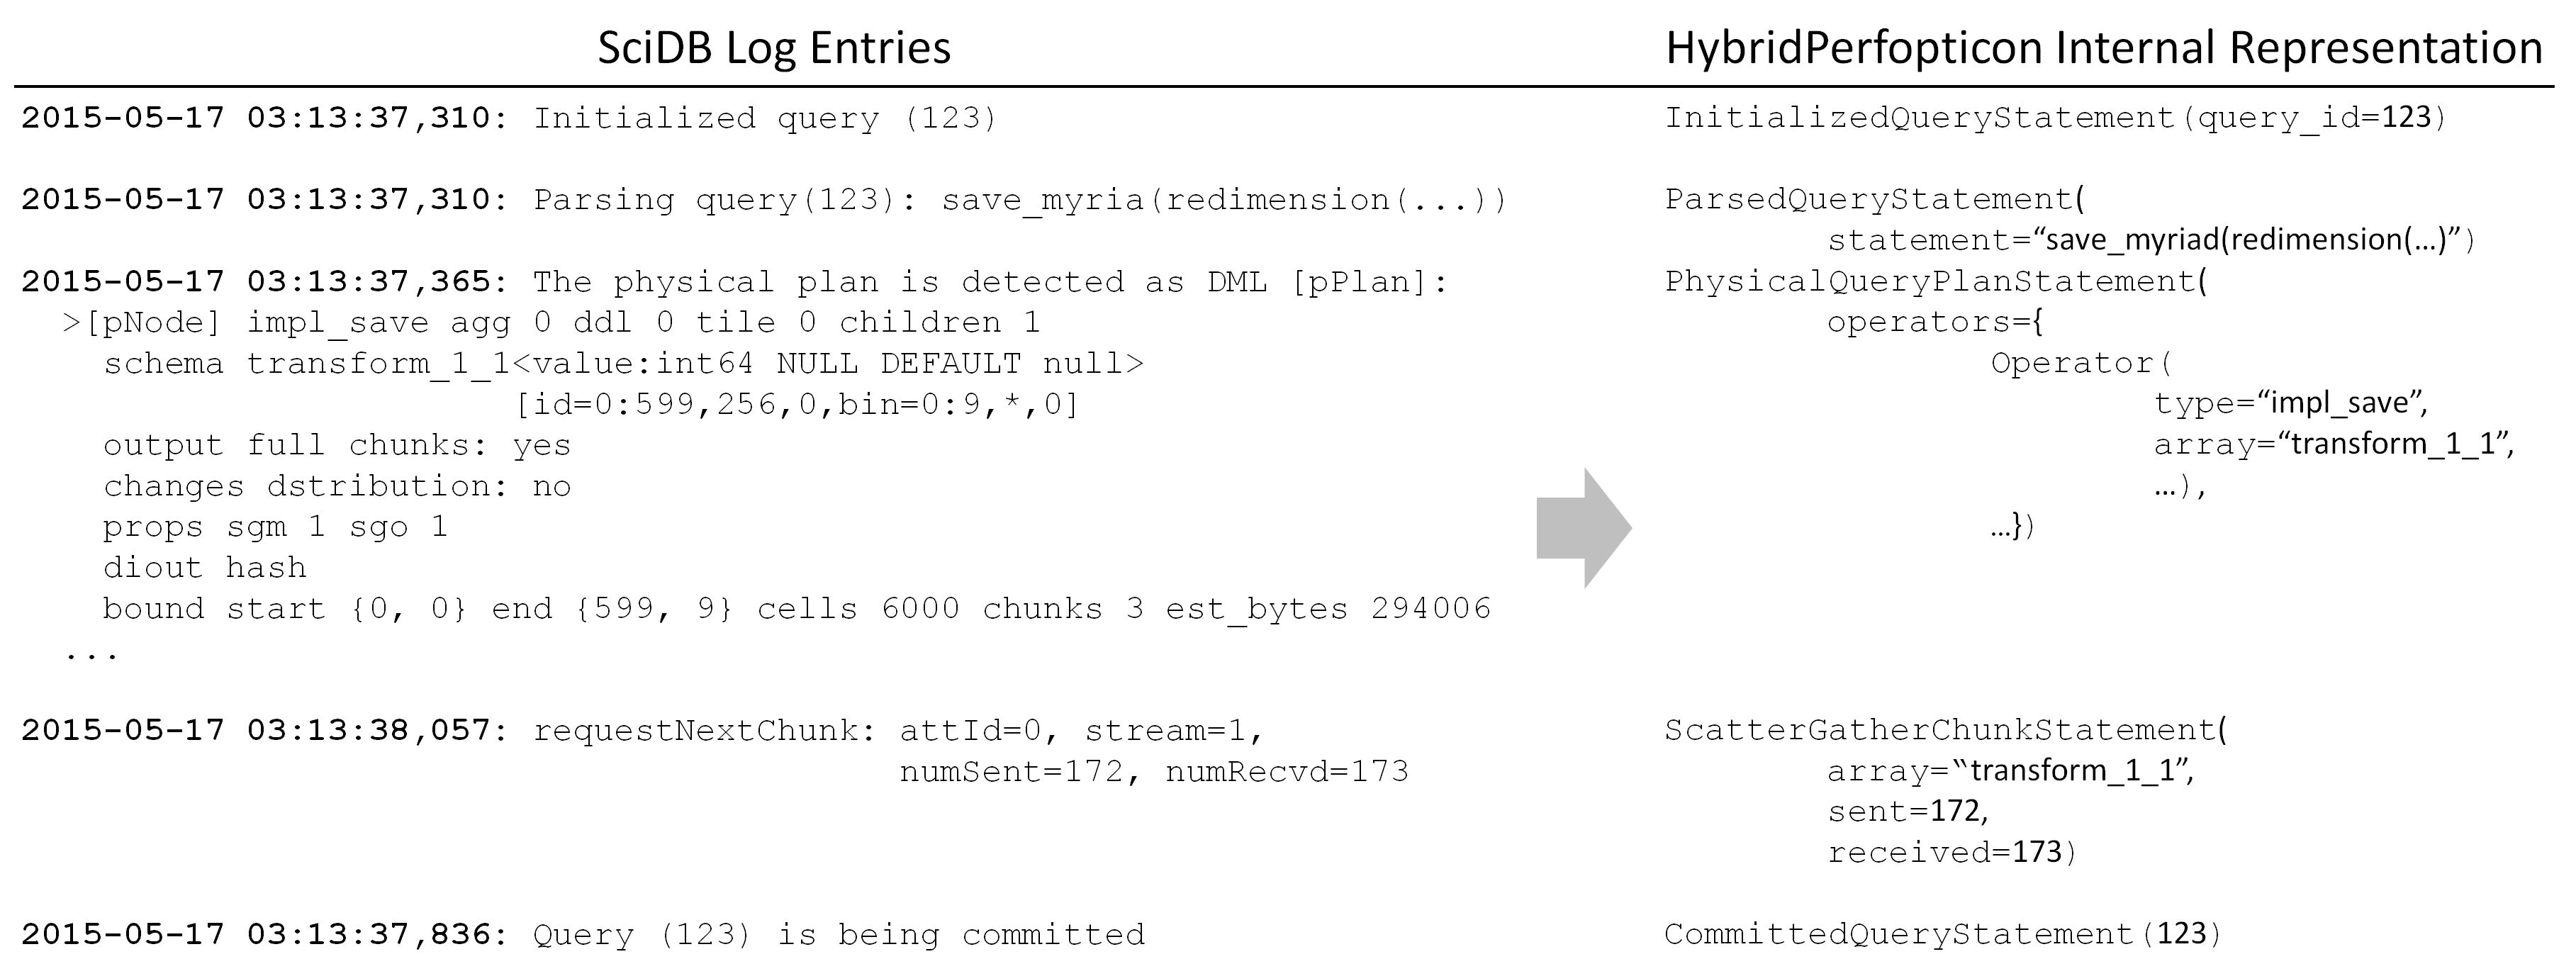
\includegraphics[width=\textwidth]{log-representation.png}
\caption{SciDB log fragment (abbreviated for readability) and mapped equivalents in the HybridPerfopticon HTTP server}
\label{fig:scidb-log-example}
\end{figure*}

Our first task was to expose similar functionality targeted at the SciDB DBMS.  While we could take a similar route in SciDB by instrumenting each operator and responding to aggregation requests, this would be a time-consuming task and would decrease the performance of SciDB itself.  Instead, we elected an alternative approach: since the relevant profiling metadata is already present in the SciDB logs, we generated our performance metrics by scraping these log files.  While this resulted in decreased performance on startup\footnotemark, our approach has the added benefit of requiring no changes to the SciDB source code.  We expect that this approach would allow for a low-barrier introduction of similar systems, assuming that the salient metrics already exist in the log files.

\footnotetext{Approximately ten seconds per 100MB of logging data.}

The architecture of our log-scraping process is illustrated in Figure \ref{fig:scidb-log-parsing}.  The entry point to this process is the \texttt{SciDBParser} class, which is responsible (via the \texttt{SciDBLog} class) for converting raw log entries into sequences of statements.  Statements associated with a given query are aggregated into a physical plan, and the operators for that plan are identified and hierarchically assembled within that plan.  During the log interpretation process we also identify performance metrics associated with each executed query and associate those results with the plan.

An illustration of the log-scraping process is listed in Figure \ref{fig:scidb-log-example}.  In this log fragment (abbreviated for readability), the \texttt{SciDBLogParser} identifies the beginning of the query execution process, identifies (and interprets) the associated physical plan, associates a scatter/gather operation with an underlying operator, and notes the time at which the query is committed.  Each of these entries are converted into an equivalent statement, and the useful metadata for each statement is embedded therein.



\begin{figure}[h]
\begin{center}
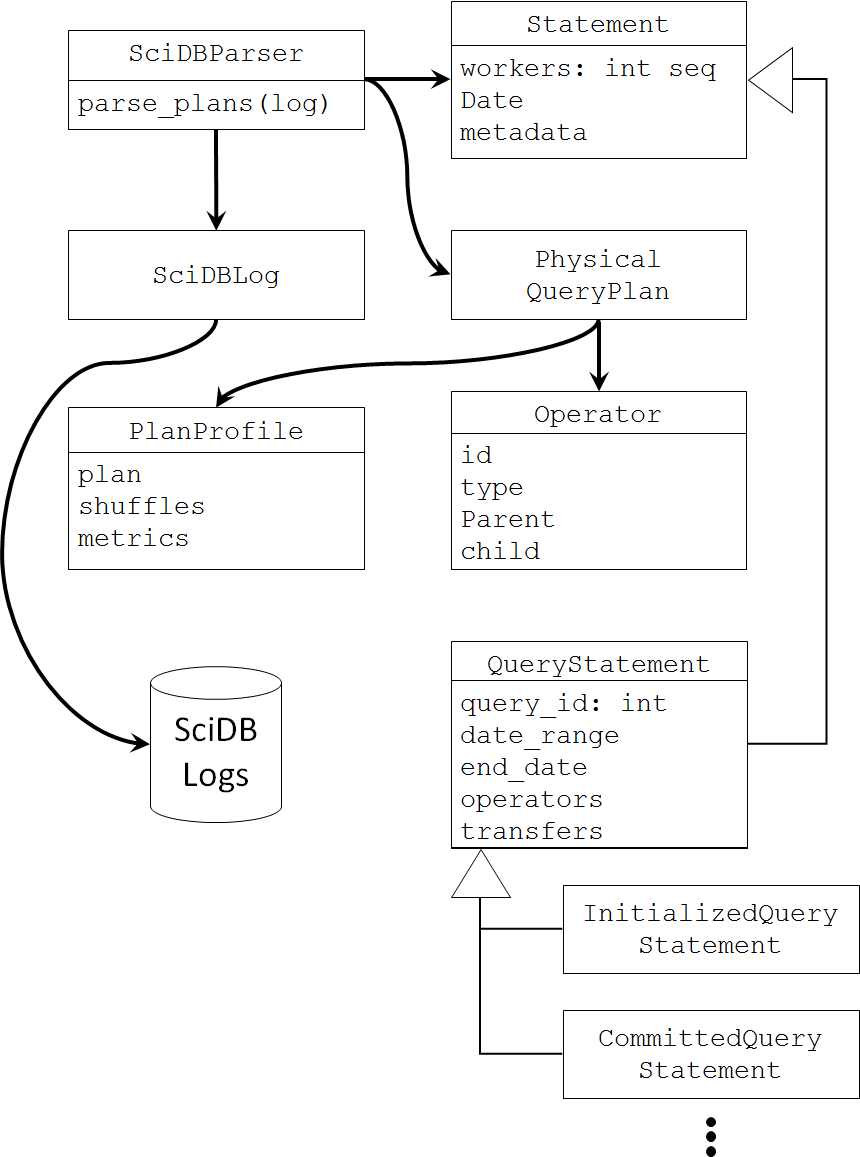
\includegraphics[scale=0.25]{log-scraping.png}
\end{center}
\caption{Architecture of the SciDB log parsing components.}
\label{fig:scidb-log-parsing}
\end{figure}


\subsection{Extending Perfopticon to Support Additional DBMSs}

In order to extend Perfopticon to support queries across multiple DBMSs, we first explored the use of existing extension points.  Since Perfopticon is not designed to be directly extendable (\eg, via a plugin-style architecture), extensive modification to the framework would be required to support the kinds of hybrid plans we intended to visualize.  Instead, we elected an alternative approach where a substantial portion of the necessary logic was hidden behind the HTTP server (our "hybrid HTTP server", described in detail below) to which Perfopticon connects for plan and profiling metadata.

While this approach greatly reduced the modifications required to realize our desired functionality, some changes were nonetheless required to Perfopticon itself.  For example, it is necessary to be able to identify the system of origin for each plan fragment; this is important not only for visualization purposes (e.g., to color fragments by system type) but also functionally.  For example, the hybrid HTTP server must know from which system a fragment originated in order to retrieve correct profiling metrics.

A number of similar minor modifications were required throughout the Perfopticon framework.  By way of example, SciDB fragments required a SciDB-specific query identifier be attached to each fragment; we envision that additional metadata would be required in order to support other systems.  For example, in a graph-oriented DBMS it might be useful to associate a range of vertex identifiers operated on by a given operator.

\subsection{Hybrid HTTP server}

Given that HybridPerfopticon continues to expect HTTP responses in the same form as Perfopticon, our hybrid HTTP server needed to do a substantial amount of manipulation to compose hybrid plans without violating this requirement.  A high-level architectural overview of our approach is illustrated in Figure \ref{fig:hybrid-architecture}.

For each incoming request, our server first distinguished between three cases:

\begin{itemize}
\item \textbf{Hybrid requests}.  When a request for a hybrid plans is received, copies of the associated Myria and SciDB plans are retrieved (the former via the Myria REST endpoint).  These plans are then combined into a Perfopticon-compatible format using the algorithm described in simplified form in Algorithm \ref{alg:create-hybrid-plan}.  Note that this process (i) attaches a system of origin to each fragment, (ii) concatenates all fragments into a flattened list, and (iii) ensures that parent/child relationships are established between fragment pairs having different origin systems.
\item \textbf{Myria requests}.  When we receive a request for Myria-specific, non-hybrid resources (e.g., metadata about a relation that exists only on the Myria DBMS), we issue a 301 redirect to the Myria REST server.  This enables the hybrid HTTP server to be the sole communication endpoint for HybridPerfopticon without our needing to choose between two URLs on the client side.
\item \textbf{SciDB requests}.  Requests for SciDB profiling data (e.g., the execution time offsets for a SciDB subquery) directly leveraged the plan and profiling logic described above; responses for these requests utilized a schema that conformed precisely to their Myria counterparts.
\end{itemize}

\begin{figure}[h]
\begin{center}
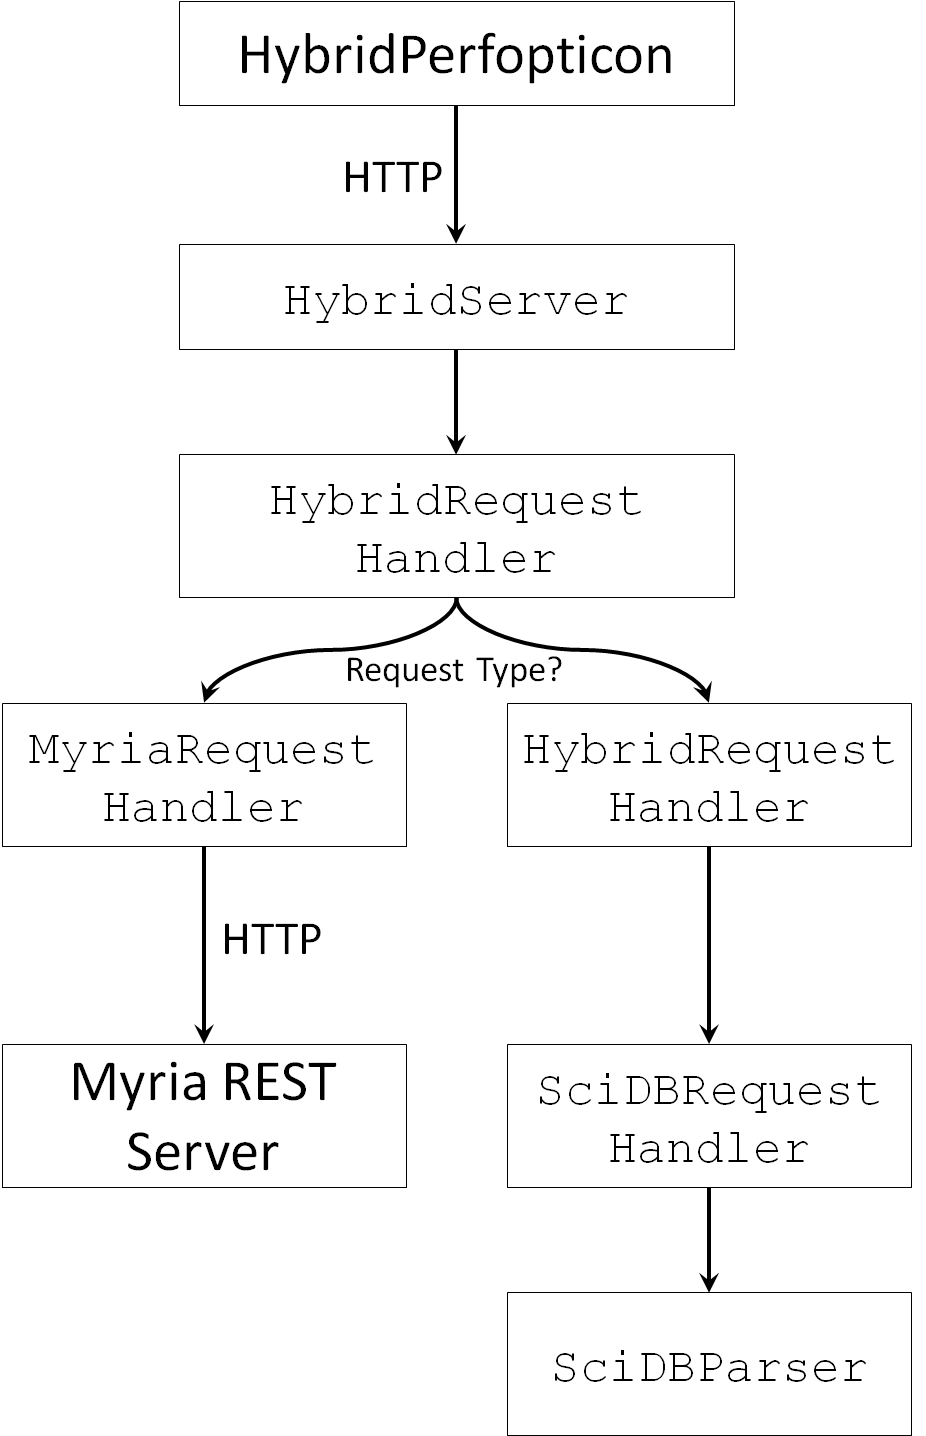
\includegraphics[scale=0.15]{hybrid-server-architecture.png}
\end{center}
\caption{Architecture of the HTTP server that aggregates plans from each database system and returns a (combined) hybrid plan.}
\label{fig:hybrid-architecture}
\end{figure}

\begin{algorithm}
\caption{Combining Myria and SciDB plans}\label{alg:create-hybrid-plan}
\begin{algorithmic}[1]
\Statex{\hspace{-.15in}{\bf function} \textsc{create-hybrid-plan}($id$, $url_{\textsc{myria}}$)}
\State plan = \texttt{HTTP-GET}($id$, $url_{\textsc{myria}}$)
\For{\textbf{each} $\text{fragment}_{\textsc{Myria}}$ $\in$ plan}
  \State $\text{fragment}_{\textsc{Myria}}$.origin = "Myria"
  \For{\textbf{each} $\text{op}_{\textsc{Myria}}$ $\in$ $\text{fragment}_{\textsc{Myria}}$}
    \If{$\text{op}_{\textsc{Myria}}$.type is \texttt{SciDBScan}}
      \State $\text{plan}_{\textsc{SciDB}}$ = load($\text{op}_{\textsc{Myria}}$.parent.id)
      \For{\textbf{each} $\text{fragment}_{\textsc{SciDB}}$ $\in$ $\text{plan}_{\textsc{SciDB}}$}
		\State $\text{fragment}_{\textsc{SciDB}}$.origin = "SciDB"
        \State plan.fragments += $\text{fragment}_{\textsc{SciDB}}$
        \For{\textbf{each} $\text{op}_{\textsc{SciDB}}$ $\in$ $\text{fragment}_{\textsc{SciDB}}$}
          \If{$\text{op}_{\textsc{SciDB}}$.type is \texttt{MyriaSave}}
          	\State $\text{op}_{\textsc{SciDB}}$.child.id = $\text{op}_{\textsc{Myria}}$.id
          \EndIf
        \EndFor
	  \EndFor
    \EndIf
  \EndFor
\EndFor

\State return plan

\end{algorithmic}
\end{algorithm}

\section{Results}


\begin{figure*}
\centering
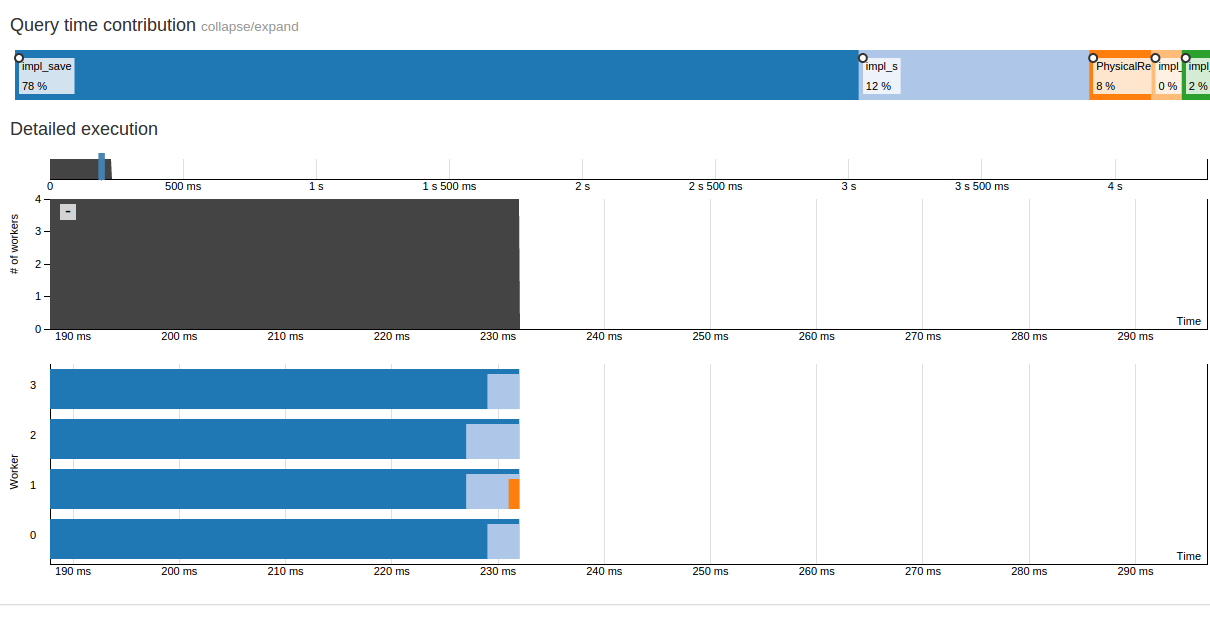
\includegraphics[width=\textwidth]{visualization-detail.png}
\caption{Detailed profiling results for the SciDB fragment in Figure \ref{fig:hybrid-visualization}.}
\label{fig:scidb-detail}
\end{figure*}

We now present an overview of our visual encoding choices and the visualization extensions present in HybridPerfopticon by introducing a sample hybrid use-case. In our example, a user first inputs the hybrid query identified in figure \ref{fig:hybrid-plan}. This query is first performs a redimension in SciDB and then transmits the resulting dataset to Myria.  The Myria DBMS then performs a join operation and stores a projection of the result. 

Figure \ref{fig:hybrid-visualization} shows the hybrid visualization for this query. Note that we distinguish the origin of each fragment by color.

\begin{figure}[h]
\begin{center}
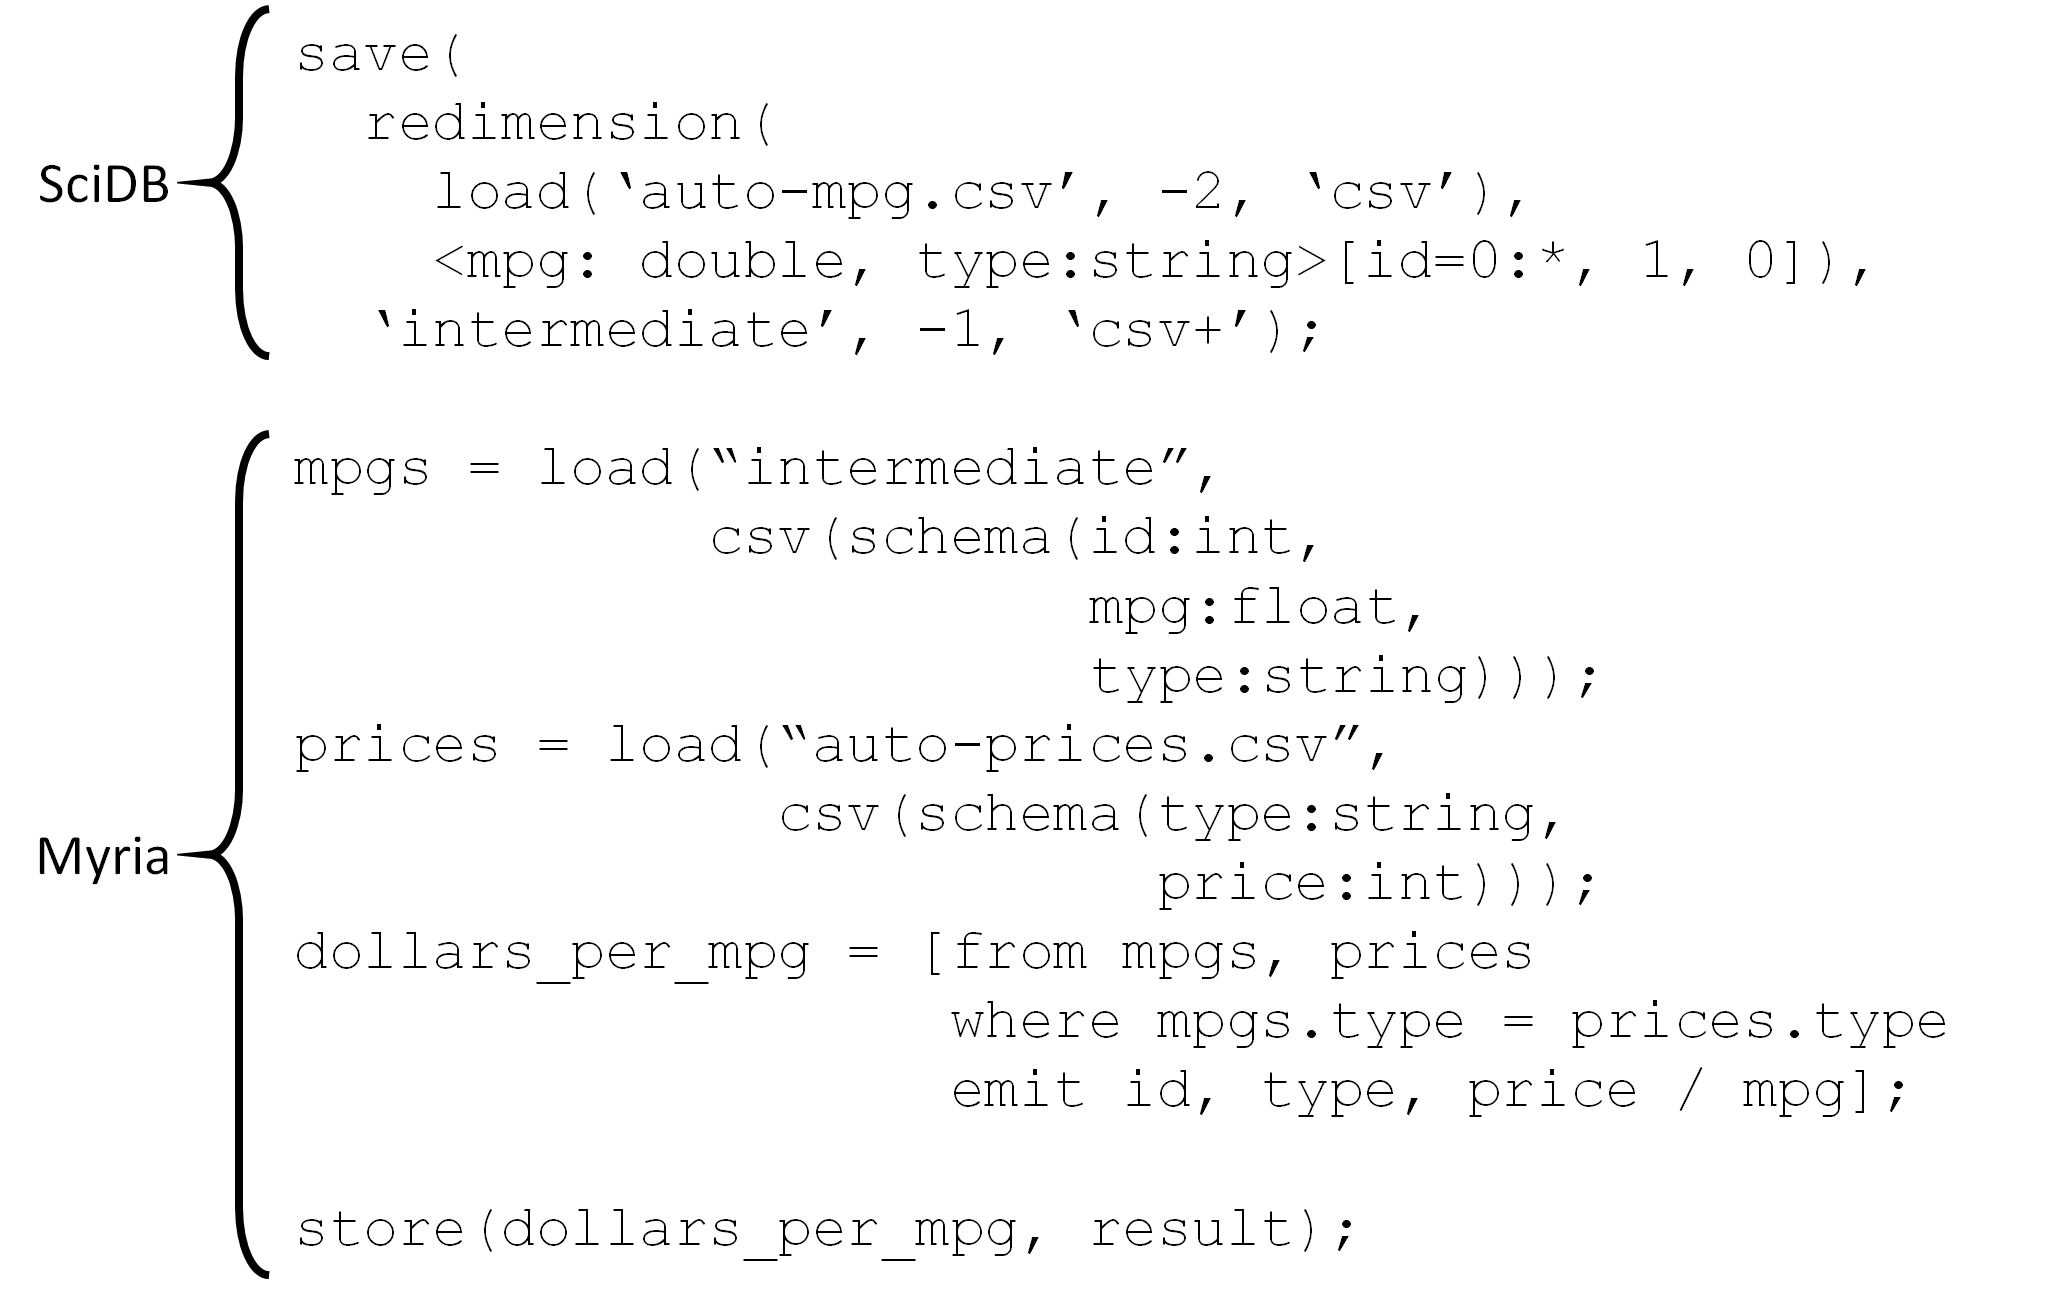
\includegraphics[scale=0.17]{visualization-query.png}
\end{center}
\caption{A hybrid query used as input to HybridPerfopticon.  See Figure \ref{fig:hybrid-visualization} for generated hybrid plan.}
\label{fig:hybrid-plan}
\end{figure}

\begin{figure}[h]
\begin{center}
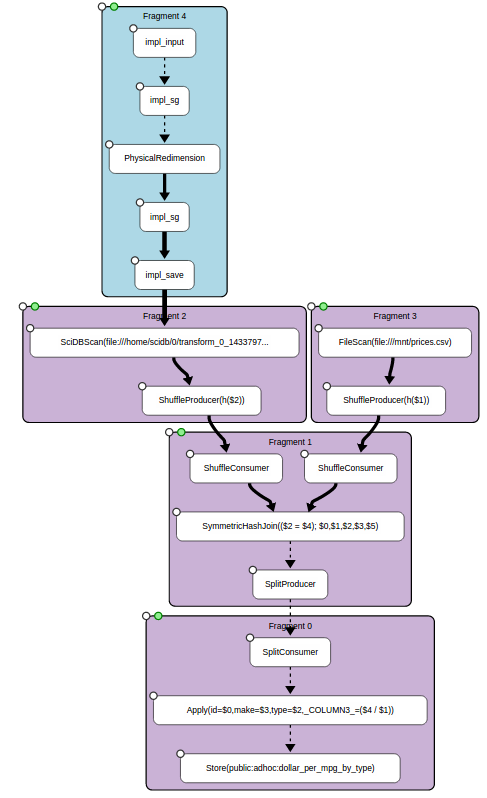
\includegraphics[scale=0.4]{visualization-example.png}
\end{center}
\caption{A hybrid plan as visualized by HybridPerfopticon.  This hybrid query begins with a SciDB scan/redimension, after which the resulting array is transferred to Myria for joining on a second dataset.}
\label{fig:hybrid-visualization}
\end{figure}

Since SciDB treats each query as being fully independent, each part of the hybrid query  executed on SciDB is represented as a single fragment. Should the input query have had multiple, potentially-interleaved SciDB queries, we would have seen additional SciDB fragments in the resulting hybrid plan visualization. 

As with Perfopticon, a user can select individual fragments and get detailed profiling views.  This is illustrated in Figure \ref{fig:scidb-detail}. The hybrid HTTP server which serves the plans also returns profiling API requests and automatically reconciles differences between SciDB and Myria fragments. 

The next feature added to HybridPerfopticon involves the animation of the query plan by showing tuple- and array element-flow across different operators at various points in query execution process. This is shown to the user by animating the size of the connecting arrows, and adjusting those sizes during the playback process. The idea here is to give a global perspective of how elements are being processed in the hybrid query, with the intention that a user will quickly identify areas of interest for subsequent drill-down.

\begin{figure}[h]
\begin{center}
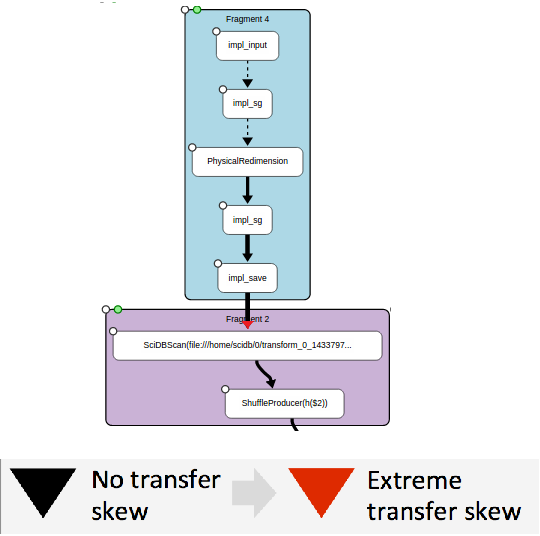
\includegraphics[scale=0.5]{skew.png}
\end{center}
\caption{Visualizing skew in inter-database transfers}
\label{fig:skew}
\end{figure}

Our final extension in HybridPerfopticon involved illustrating inter-database transfer skew.  In our display, skew is binned, color-encoded and displayed as a (normalized) mean over the previous two seconds.  This running average is important to minimize rapid fluctuation which are both distracting and serve to conceal the far more important global patterns of skew that occur in this class of queries. 

%We would like to point out that animation for very large queries lags a bit due to many API calls to the hybrid plan server. We are exploring possible ways to fix this. 

\section{Conclusions \& Future Work}

In this work we described HybridPerfopticon, a visualization tool for hybrid queries that cross DBMS boundaries.  A tool that does so is critically needed, especially given that the performance profiles of this class of queries are not well-understood.  Accordingly, we expect that this tool will serve as a useful means by which the hybrid DBMS space may be explored.

While our approach of using existing log files to generate performance metrics is certainly not novel, the use of log file parsing to quickly add a second DBMS to a query visualization framework represents an opportunity to extend the reach of HybridPerfopticon to a wide-ranging set of systems.  Future work should evaluate the applicability of this approach, and if generalizable, additional attention should be paid to identifying the optimal interface by which logging metadata may be exposed to HybridPerfopticon.

However, while our log-parsing approach allowed us to quickly expose profiling data for a second DBMS inside HybridPerfopticon, more work remains to be done.  In particular, the hybrid HTTP server needs a far more robust caching subsystem; in particular, increasingly large logging files will quickly lead to an intractable startup time.  This would be easily remedied by ensuring that the results of the parsing operation were themselves logged to a DBMS for quick subsequent retrieval.

Additionally, future work should evaluate how to best degrade in the face of differing levels of profiling granularity.  For example, we were able to produce SciDB profiling metrics at the millisecond level, whereas Myria profiles at nanosecond granularity.  A hybrid visualization framework should be able to gracefully reconcile both; similarly, we expect that some systems will not have support for some profiling areas and that the framework should evolve to gracefully handle these cases.

Finally, given that we hypothesize that hybrid queries will tend to be larger than their single-database counterparts, it may be the case that the resulting plans with numerous fragments are not easily navigated in the HybridPerfopticon system.  Follow-on work should explore whether these fragments can be combined into larger groupings, either by database system type or (better yet) by grouping fragments by higher-level function.

\bibliographystyle{abbrv}
\bibliography{bibliography}

\end{document}
